% !TEX root = hazelnut-dynamics.tex
\newcommand{\examplesSec}{Live Programming in Hazel}
\section{\examplesSec} 
\label{sec:examples}

% !TEX root = hazelnut-dynamics.tex

\begin{figure}[t]
\begin{subfigure}[t]{\textwidth}
\centering
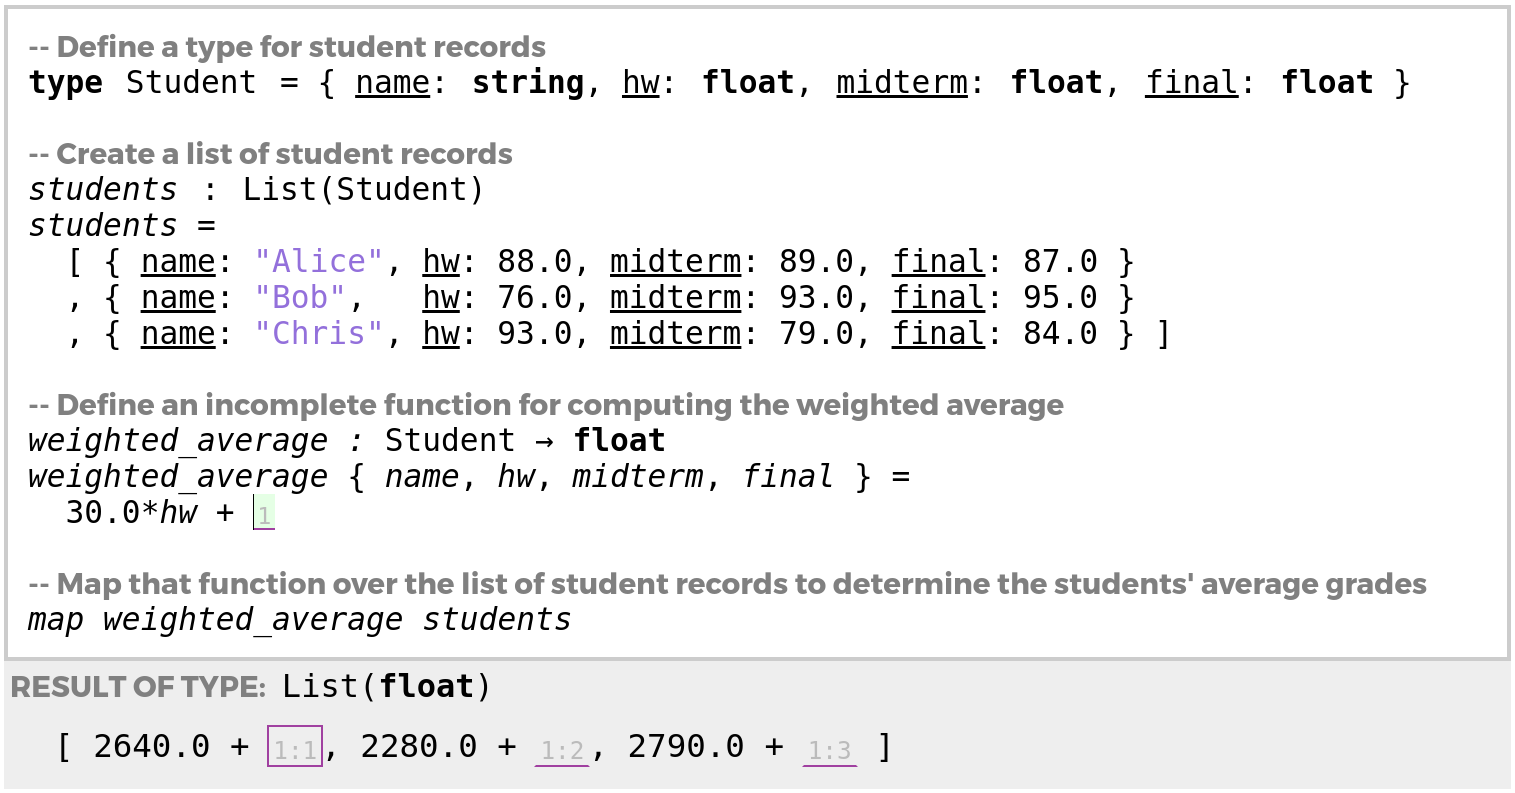
\includegraphics[width=0.8\textwidth,interpolate=false]{images/grades-cell-mockup.png}
\vspace{-3px}
\caption{Evaluating an incomplete functional program past the first hole}
\label{fig:grades-cell-mockup}
\end{subfigure}

\vspace{10px}

\begin{subfigure}[t]{\textwidth}
\centering
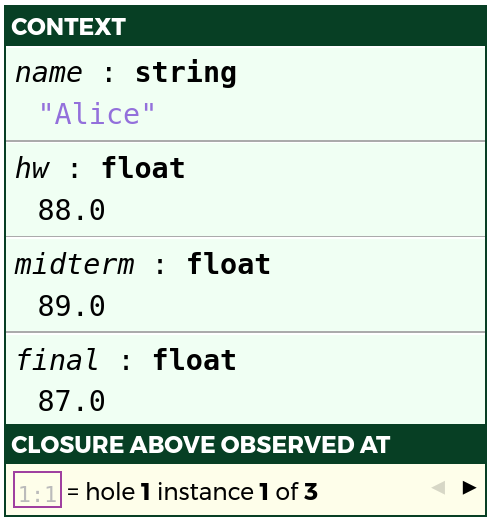
\includegraphics[width=0.29\textwidth,interpolate=false,valign=c]{images/grades-sidebar-1.png}
~${}^\blacktriangleright$
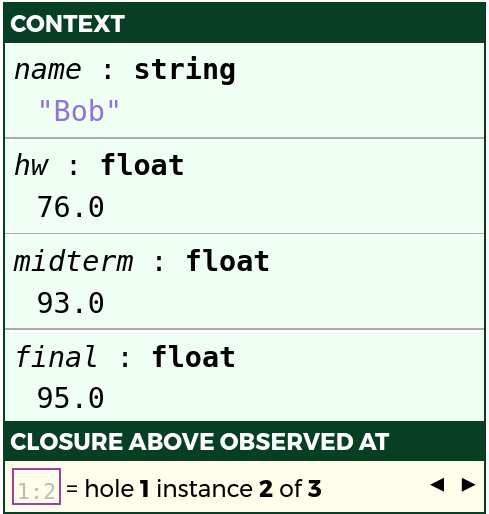
\includegraphics[width=0.29\textwidth,interpolate=false,valign=c]{images/grades-sidebar-2.png}
~${}^\blacktriangleright$
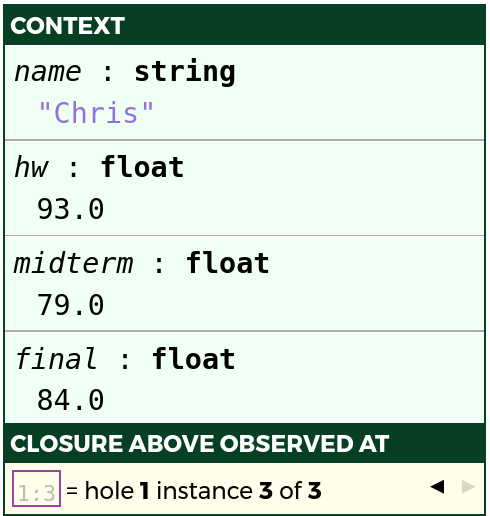
\includegraphics[width=0.29\textwidth,interpolate=false,valign=c]{images/grades-sidebar-3.png}
\caption{The live context inspector communicates relevant static \emph{and} dynamic information about variables in scope.}
\label{fig:grades-sidebar}
\end{subfigure}
% %% TODO once the code above is removed, scale up the screenshots
% 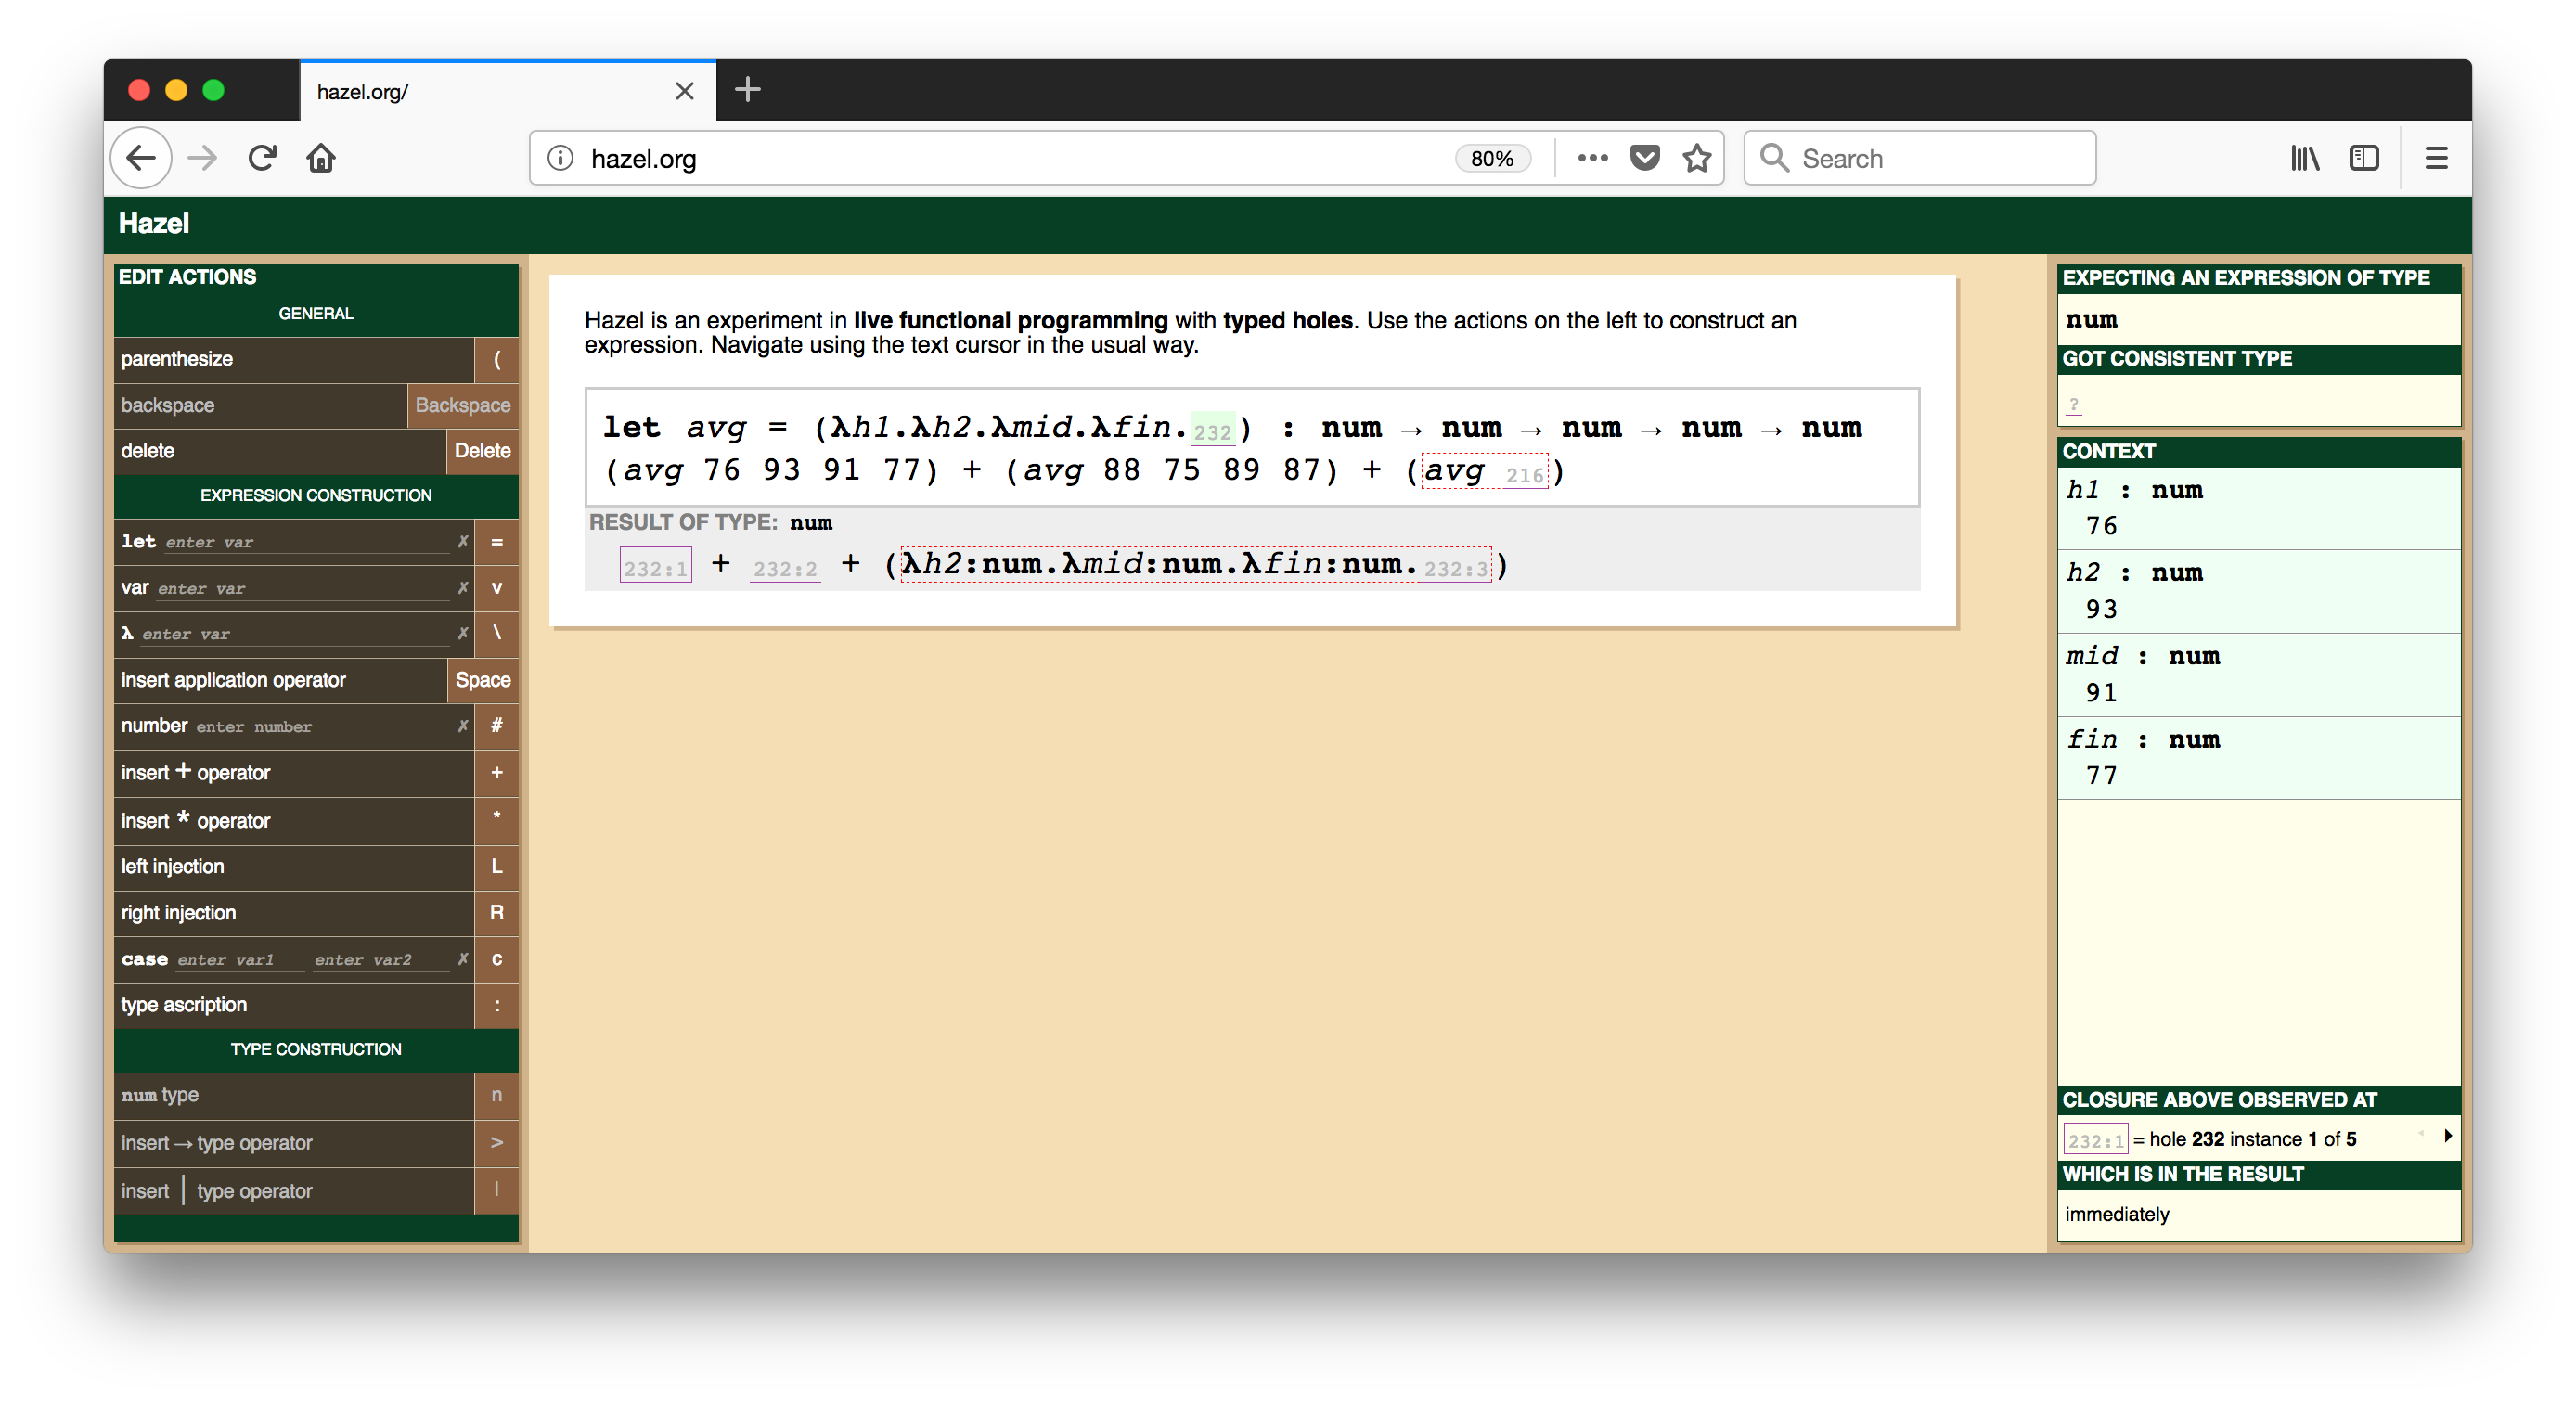
\includegraphics[scale=0.20]{images/hazel-placeholder-0.png}

% \rkc{Draw arrows and captions on the top figure to show how to get
% to the bottom figure.
% ser navigates to hole a, types + to create a plus, types * to create a
% multiplication, types \#10 to create 10, types vh1 to create variable use.}

% 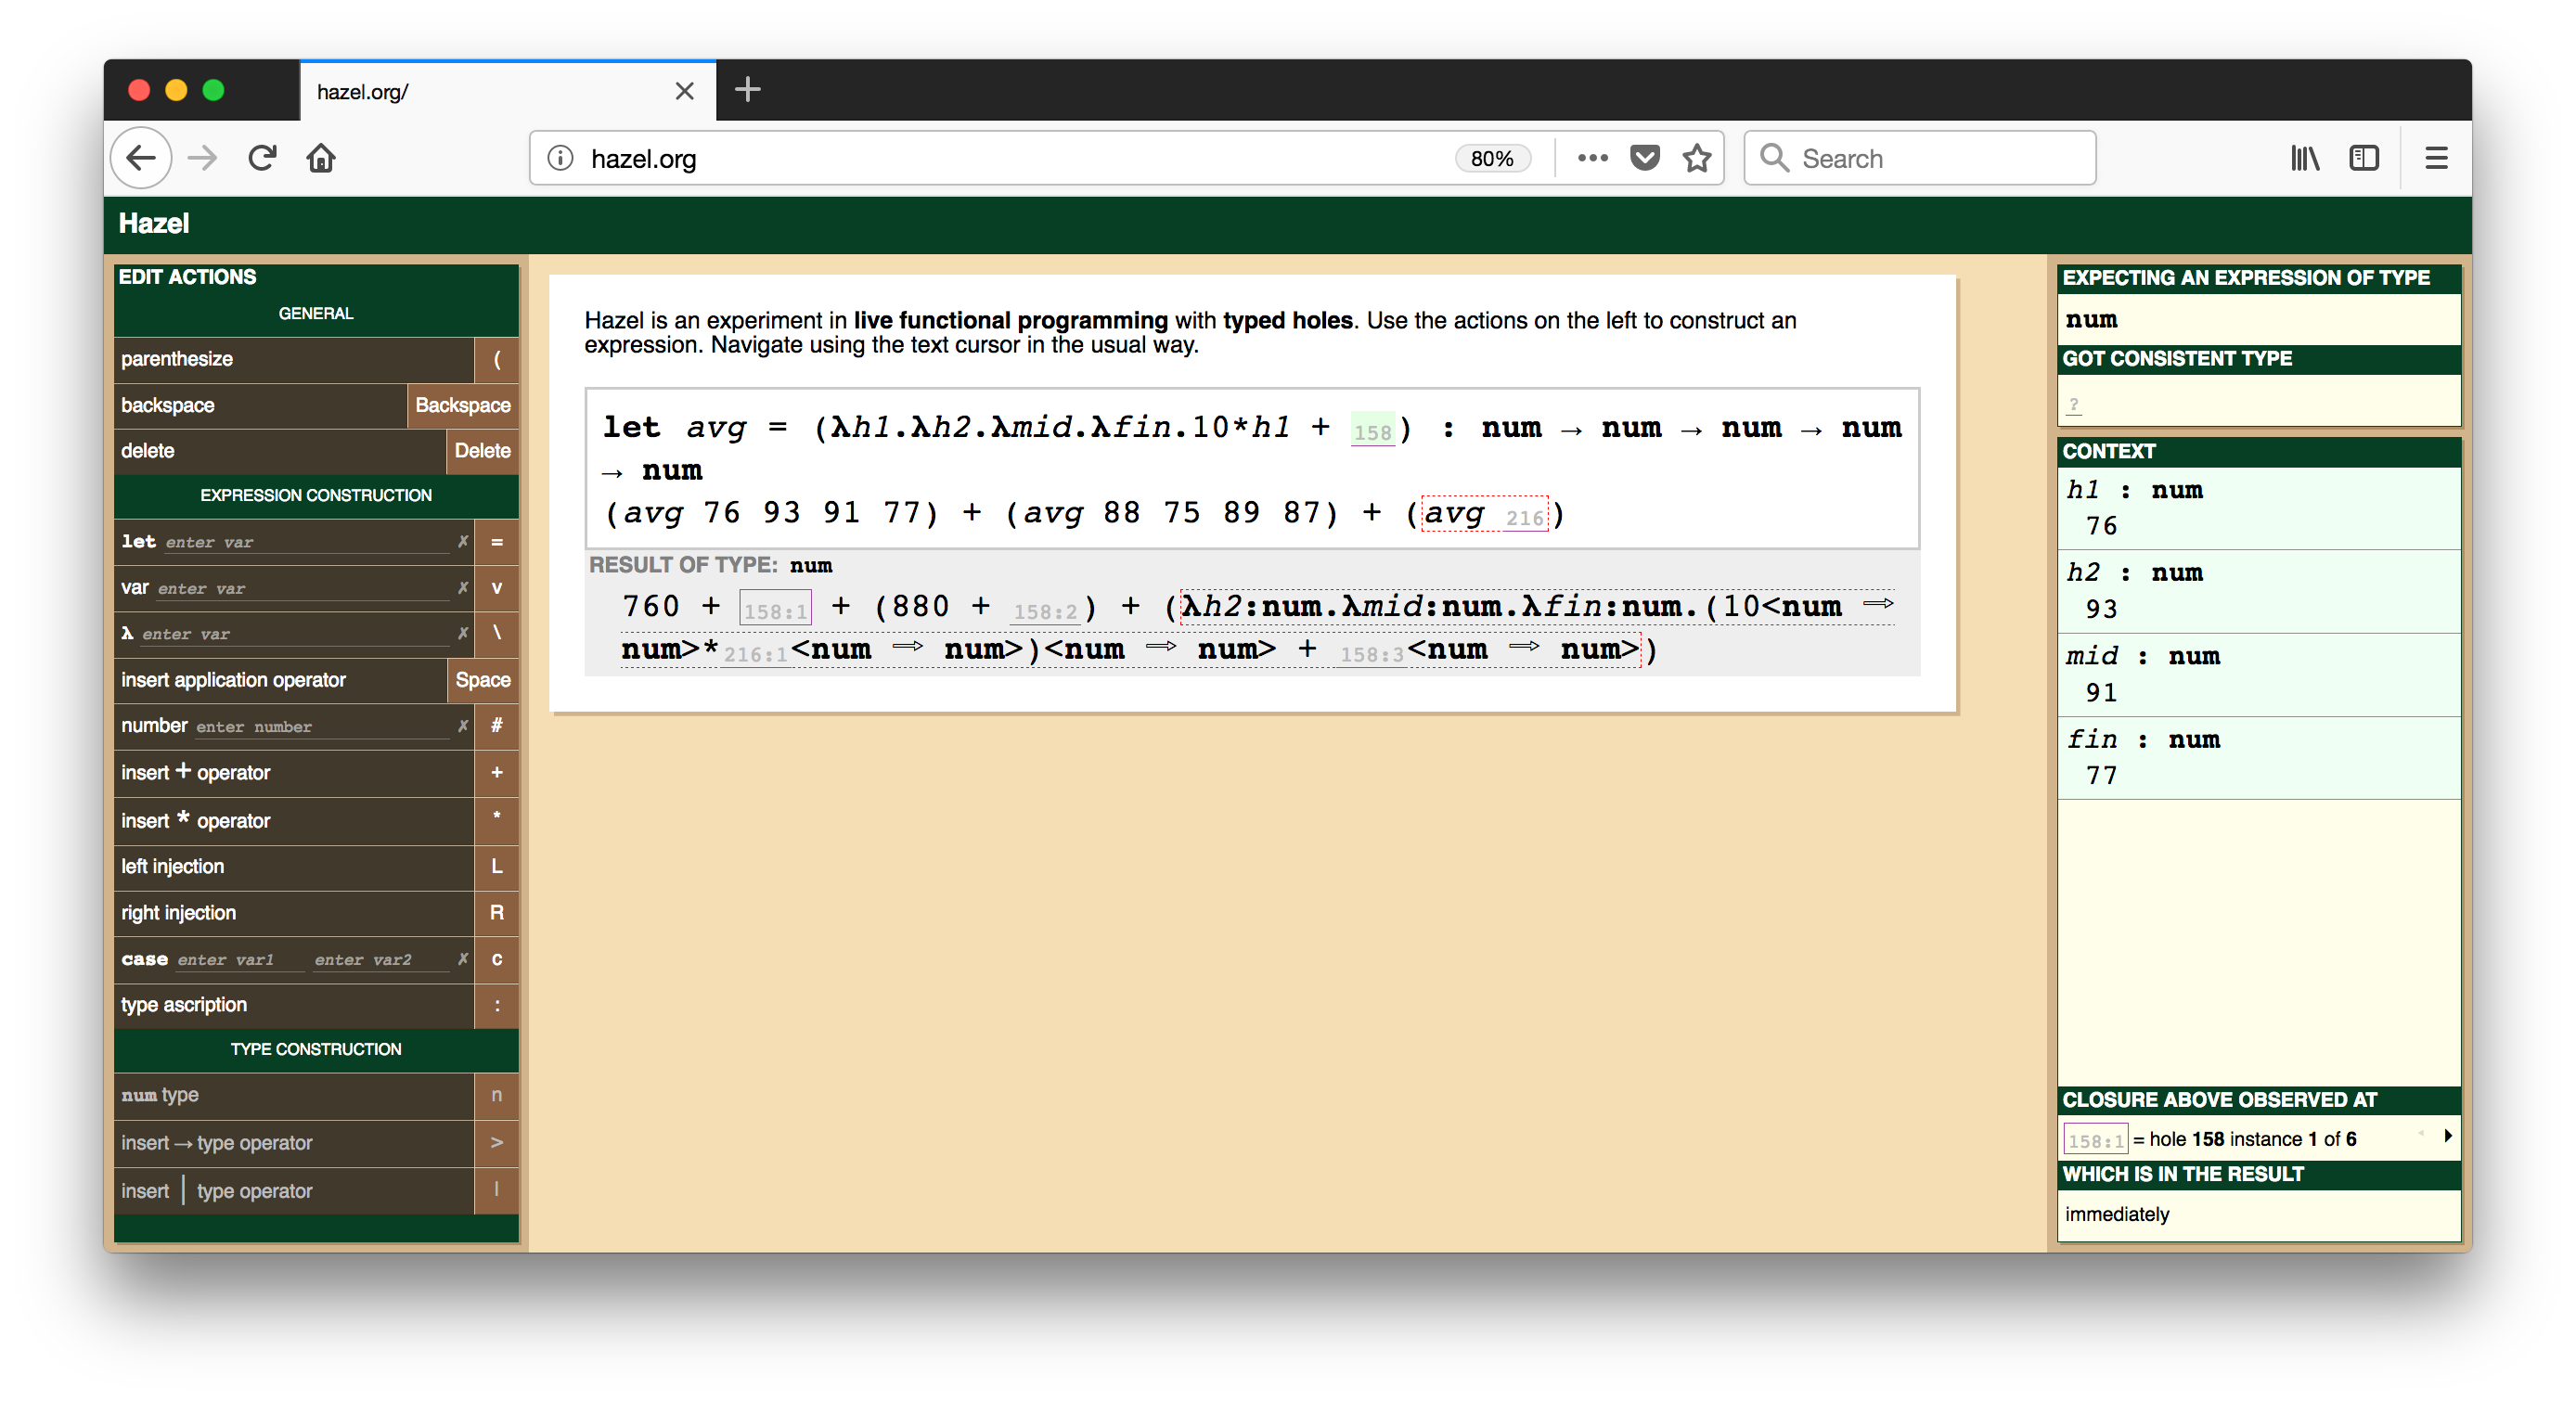
\includegraphics[scale=0.20]{images/hazel-placeholder-1a.png}
\vspace{3px}

\caption{Example 1: Grades}
\label{fig:grades-example}
\vspace{-5px}
\end{figure}



\newcommand{\overviewExample}[2]{\paragraph{Example {#1}: {#2}}}

Let us start with an example-driven overview of this paper's approach in \Hazel, a live programming environment being developed by \citet{HazelnutSNAPL}. The \Hazel user interface is based roughly on IPython/Jupyter \cite{PER-GRA:2007}, with a result appearing below each cell that contains an expression, and the \Hazel language is tracking toward feature parity with \Elm~(\url{elm-lang.org}) \cite{czaplicki2012elm,Elm}, a popular pure functional programming language similar to ``core ML'', with which we assume familiarity. \Hazel is intended initially for use by students and instructors in introductory functional programming courses (where \Elm~ has been successful \cite{DBLP:journals/corr/abs-1805-05125,zhang2018graphics}). 

For the sake of 
exposition, we have post-processed the screenshots in this section after generating them in \Hazel to make use of  ``syntactic and semantic sugar'' from \Elm~that was not available in \Hazel (which, as of this writing, implements little more than the language features described in Sec.~\ref{sec:calculus} and the appendix). These conveniences are orthogonal to the contributions of this paper; all of the user interface features demonstrated in this section have been implemented and all of the computations can be expressed using standard ``encoding tricks''.

\subsection{Live Programming with Incomplete Expressions}

The process of writing new program fragments includes many states in which the
program under construction is, by definition, incomplete.
%
It is natural for a programmer to ``jump back and forth'' between different
places in the program, iteratively and alternately developing the missing
pieces.
%
The primary benefit of our approach is that such programs can be evaluated in
order to provide useful feedback during this editing workflow.

% !TEX root = hazelnut-dynamics.tex

\begin{figure}[t]
\begin{subfigure}[t]{\textwidth}
\centering
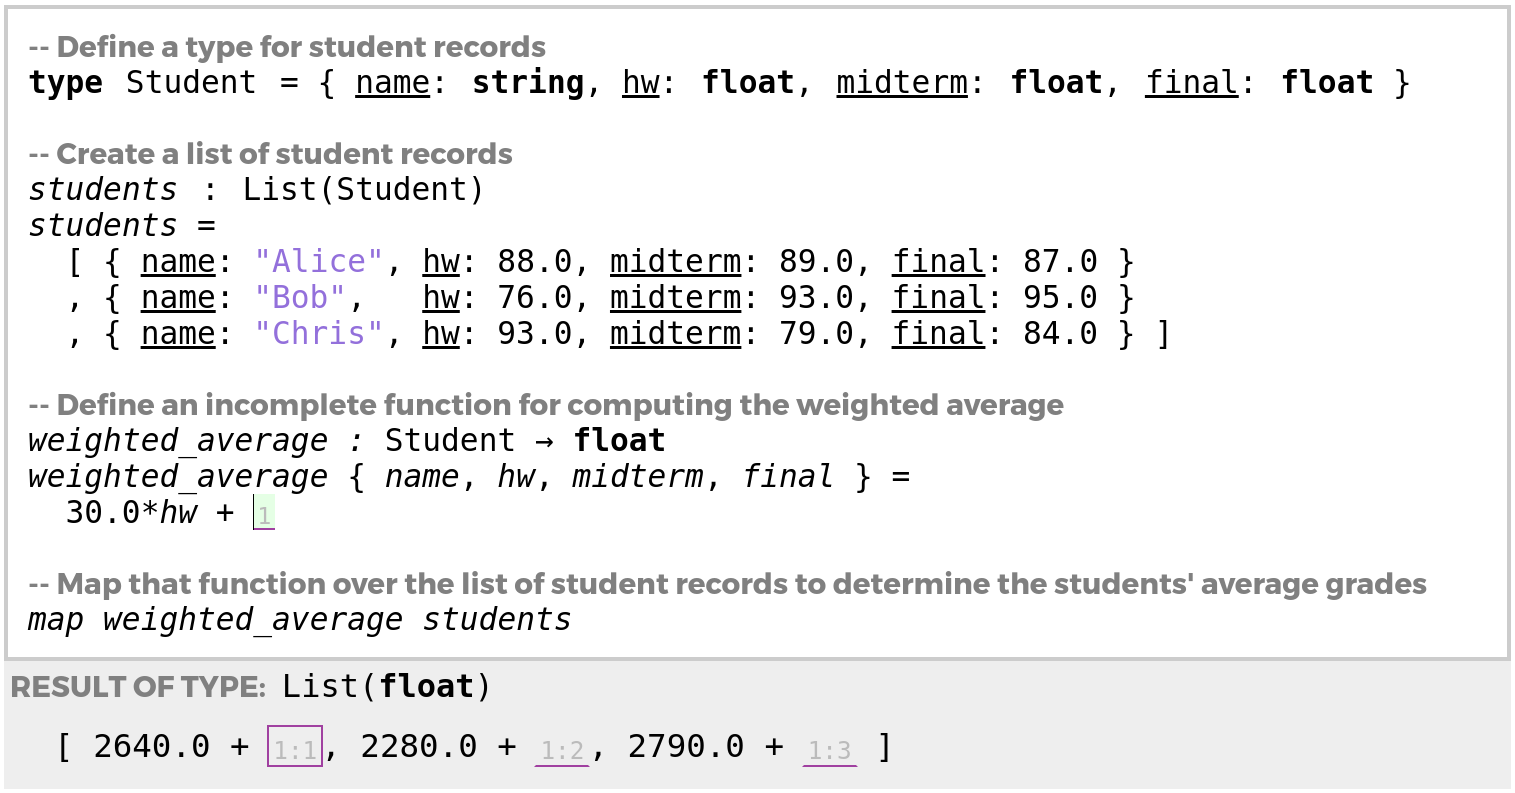
\includegraphics[width=0.8\textwidth,interpolate=false]{images/grades-cell-mockup.png}
\vspace{-3px}
\caption{Evaluating an incomplete functional program past the first hole}
\label{fig:grades-cell-mockup}
\end{subfigure}

\vspace{10px}

\begin{subfigure}[t]{\textwidth}
\centering
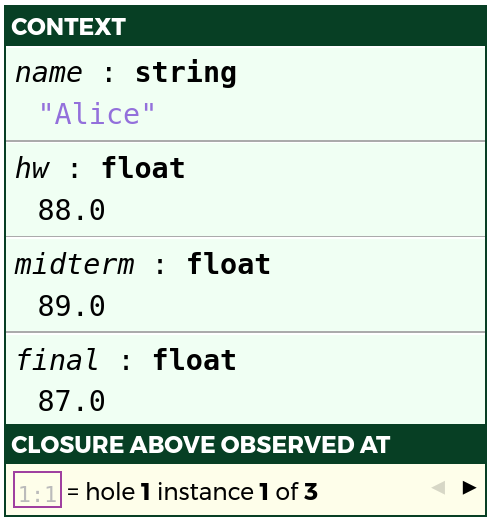
\includegraphics[width=0.29\textwidth,interpolate=false,valign=c]{images/grades-sidebar-1.png}
~${}^\blacktriangleright$
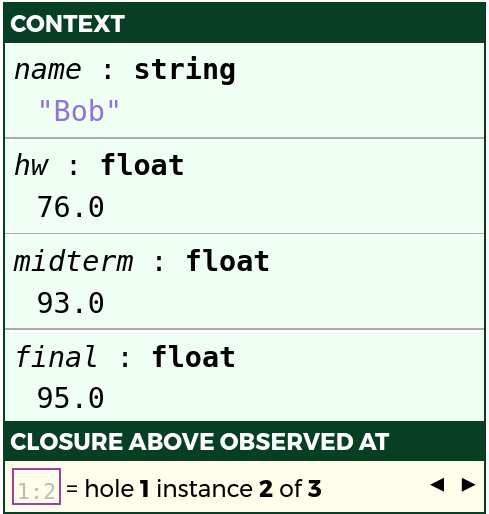
\includegraphics[width=0.29\textwidth,interpolate=false,valign=c]{images/grades-sidebar-2.png}
~${}^\blacktriangleright$
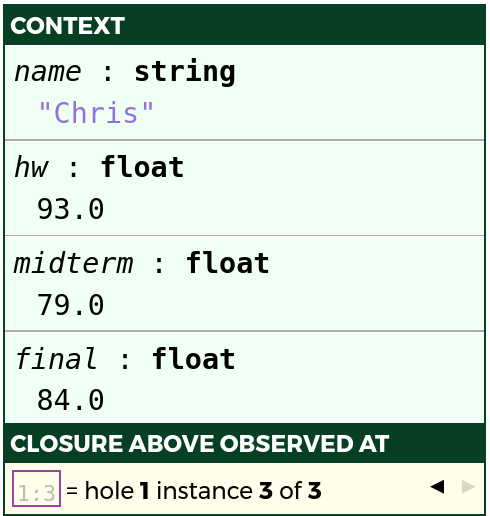
\includegraphics[width=0.29\textwidth,interpolate=false,valign=c]{images/grades-sidebar-3.png}
\caption{The live context inspector communicates relevant static \emph{and} dynamic information about variables in scope.}
\label{fig:grades-sidebar}
\end{subfigure}
% %% TODO once the code above is removed, scale up the screenshots
% 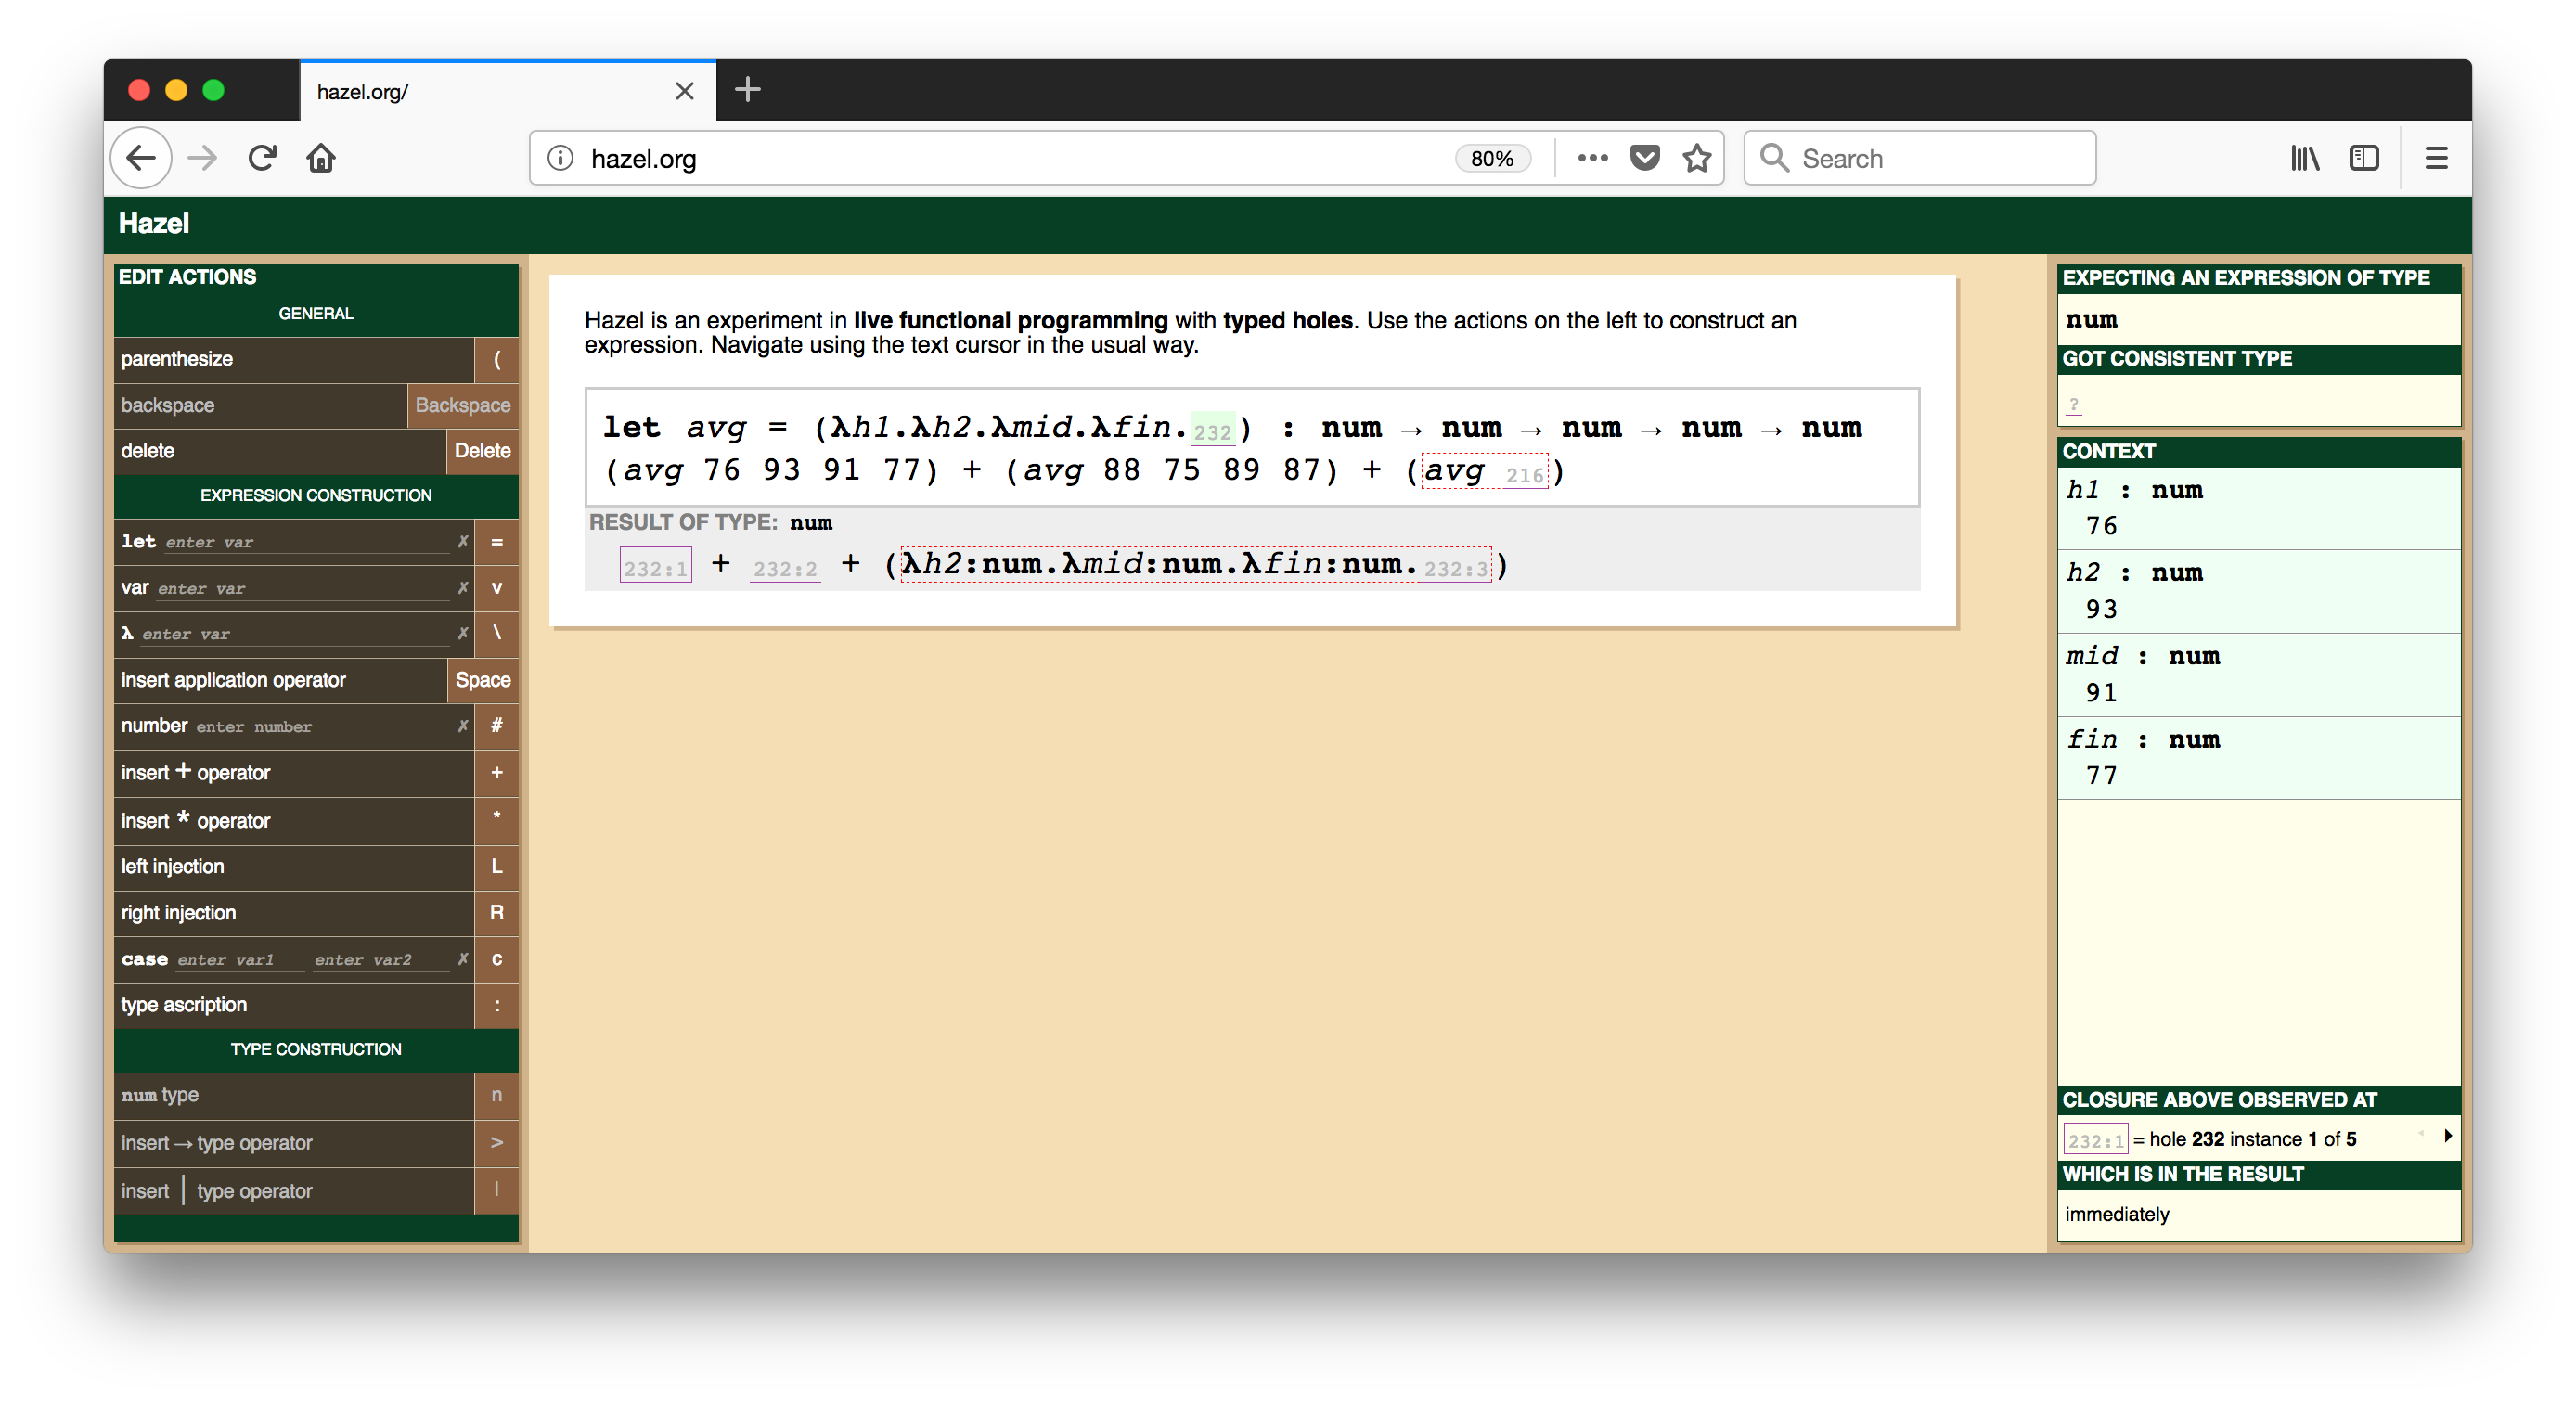
\includegraphics[scale=0.20]{images/hazel-placeholder-0.png}

% \rkc{Draw arrows and captions on the top figure to show how to get
% to the bottom figure.
% ser navigates to hole a, types + to create a plus, types * to create a
% multiplication, types \#10 to create 10, types vh1 to create variable use.}

% 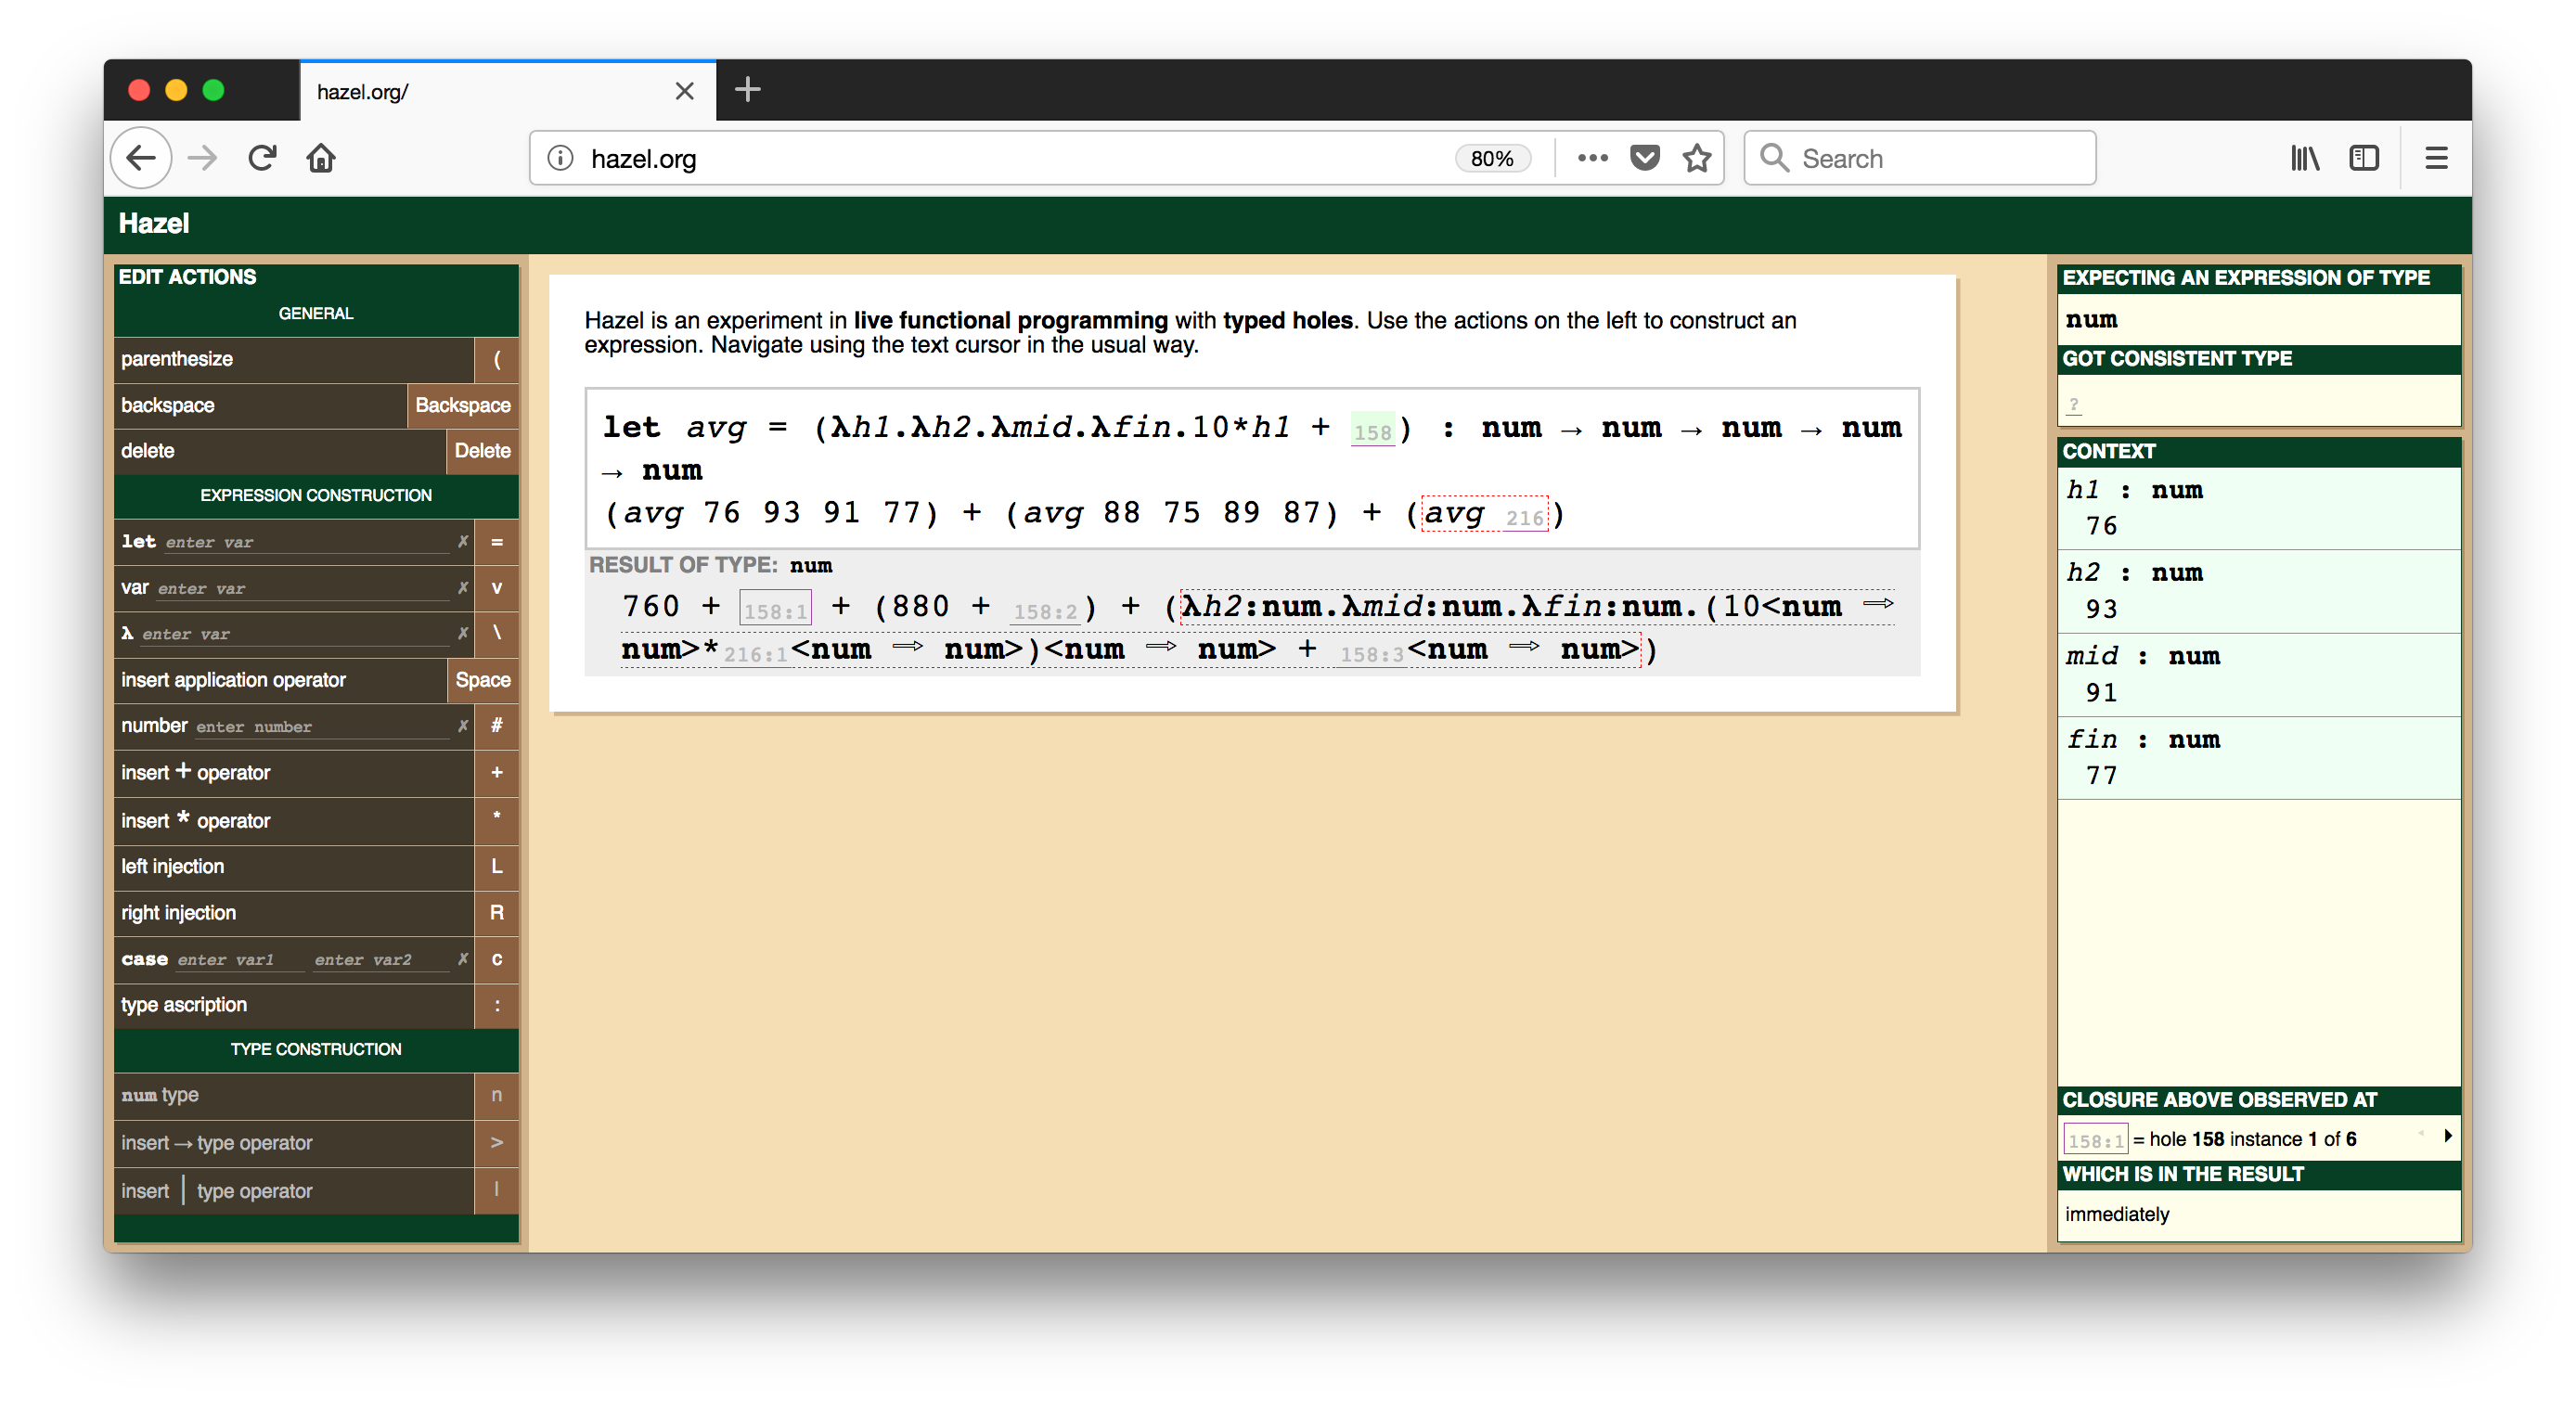
\includegraphics[scale=0.20]{images/hazel-placeholder-1a.png}
\vspace{3px}

\caption{Example 1: Grades}
\label{fig:grades-example}
\vspace{-5px}
\end{figure}


Consider a teacher who is in the midst of developing a \HazelnutLive{} notebook
(depicted in \autoref{fig:grades-example}) to compute final student grades at
the end of a term.
%
In the first cell in \autoref{fig:grades-example}, the teacher defines a record
type, \li{student_data}, for each student's course data.
%
In our simplified example, this includes the student's name, of type
\li{string}, and five grades, each of type \li{float}.

\overviewExample{1}{Computing Weighted Averages}
%
The teacher begins writing a \li{weighted_average} function that will
compute a weighted average, of type \li{float}, for each \li{student_data}
record.
%
The body of \li{weighted_average} is not yet written---marked with the
\emph{empty hole} on line \rkc{XXX}--- but the teacher jumps ahead to map the
function over the \li{grades} list.

\begin{lstlisting}
let weighted_average(g: student_data) =
  ??;

let weighted_averages = List.map weighted_average grades;
\end{lstlisting}

\noindent
%
\HazelnutLive{} evaluates this incomplete program, showing its
\emph{indeterminate} result in the sidebar on the right half of
\autoref{fig:grades-example}; this value is a list whose length is the same as
\li{grades}, where each element is the (indeterminate) result of evaluating the
hole expression inside \li{weighted_average}.
%
Notice that the hole on line \rkc{XXX} is assigned a unique static identifier
(\ie{}~\li{a}) and that the indeterminate results it produces are assigned
corresponding unique dynamic identifiers (\ie{}~\li{a.1}, \li{a.2}, etc.).
%
In contrast, the typical ad-hoc approach to simulating hole expressions, namely,
using placeholder expressions like \li{raise "Not yet implemented."}, would halt
the program as soon it is evaluated (in this case, inside the definition of
\li{List.map} when the function is applied to the first element of \li{grades}.
%
By ``evaluating around'' the hole in \HazelnutLive{}, the programmer can at
least see that the resulting expression does indeed evaluate to a list with the
correct number of (indeterminate) values.

Now the teacher returns to \li{weighted_average} to work on the missing
expression, with the goal of computing a weighted sum of each of a student's
grades.
%
The teacher uses a \HazelnutLive{} edit action to create a sum expression,
filling in the first summand by weighting the \li{hw1} score to account for 10\%
of the weighted average; the rest of the computation is a new hole expression
(\li{??_b}), yet to be filled in.

\begin{lstlisting}
let weighted_average(g: student_data) =
  (10.0 *. g.hw1) +. ??_b;
\end{lstlisting}

\noindent
%
\HazelnutLive{} immediately runs this incomplete program, displaying the updated
list of indeterminate expressions \li{[760.0 + ??_b.1, 880.0 + ??_b.2, ...]}.
%
Right away, the teacher recognizes that the values are too large; they should be
at most \li{100.0}.
%
The teacher realizes that representing percentage points as \li{float}s requires
that the constant on line \rkc{XXX} ought to be \li{0.10} instead.
%
Because of this live feedback, the teacher corrects this error right away and
avoids making similar programming errors in the rest of the calculation.
%
The teacher continues to build the rest of the arithmetic expression until it is
complete (there are no longer any expression holes), and the result of
immediately running the finished program shows that each of values in the final
result list is in the range \li{0.0} to \li{100.0}.

\overviewExample{2}{Assigning Letter Grades}
%
The teacher's next task is to map the weighted averages to the letter grades A
through F (we will consider only ``whole'' letter grades, for simplicity).
%
The \li{grade_cutoffs} record type describes the minimum cutoff for each of
these six possible grades.
%
Initially, each value in the \li{cutoffs} record is a hole.

\begin{lstlisting}
type grade_cutoffs =
  { a: float, b: float, c: float, d: float, f: float };

let cutoffs =
  { a = ??_a, b = ??_b, c = ??_c, d = ??_d, f = ??_f };
\end{lstlisting}

\noindent
%
%% initially all holes, because it will be different year-to-year based on the %
%data, differences in course difficulty, and to satisfy fairness criteria.
%
Before starting to fill in the cutoffs, the teacher jumps ahead to write a
function \li{letter_grade} that will make the connection between \li{cutoffs}
and \li{weighted_averages}.
%
Because she intends to look at the data to help select the cutoff values, the
teacher sorts the \li{weighted_averages} and then maps them to
\li{letter_grades}.

\begin{lstlisting}
let letter_grade(n: weighted_average) =
  if n >= cutoffs.a then "A" else
  if n >= cutoffs.b then "B" else
  if n >= cutoffs.c then "C" else
  if n >= cutoffs.d then "D" else
  if n >= cutoffs.f then "F" else "Incomplete";

let sorted_weighted_averages = List.sort weighted_averages;

let letter_grades = List.map letter_grade sorted_weighted_averages;
\end{lstlisting}

\noindent
%
When \HazelnutLive{} runs this program, the guard of the outermost conditional
(\li{n >= cutoffs.a} on line \rkc{XXX}), is indeterminate because \li{cutoffs.a}
is.
%
Therefore, each of the indeterminate expressions in \li{letter_grades} is the
entire expression body, albeit with different bindings for \li{n}.
%
Displaying such ``large'' indeterminate expressions can quickly consume all
available screen space, overwhelming the user with too much information.
%
\autoref{fig:XXX} shows how \HazelnutLive{} renders large indeterminate
expressions (\ie{}~anything other than ``small'' indeterminate value (a constant
or hole) or list of small values) simply as \li{..} to save space.
%
Hovering over this abbreviation (as shown in \autoref{fig:XXX} displays the full
indeterminate expression---as well as the evaluation environment that surrounds
it---as a tooltip.
%
\autoref{sec:discussion} discusses this and other user interface concerns when
trying to display useful live feedback without overwhelming the user.
%
These usability factors are beyond the scope of our work, which is to define
semantic foundations on which such user interfaces can be built.

To start deciding \li{cutoffs}, the teacher looks at the \li{weighted_averages}
sorted in descending order.
%
The data shows a natural gap between \li{92.2} and \li{89.5}.
%
So, she chooses to use \li{92.0} as the cutoff for A.
%
Resuming the computation from before, \HazelnutLive{} resolves the conditional
expressions for the first \rkc{XXX} indeterminate expressions, because each of
those \li{n} values was greater than \li{cutoffs.a}.
%
The remaining \rkc{XXX} expressions also proceeded to evaluate the first guard,
and are now indeterminate at the guard for the second conditional.

Before assigning other cutoff values, the teacher would like to get a sense of
whether this first choice is a good one.
%
She jumps ahead to to write a function that computes the distribution of letter
grades.

\begin{lstlisting}
let compute_distribution(list: list(float)) =
  let n = List.length letter_grades in
  List.map
    (\x -> (x, showPercentage (List.length (List.filter ((==) x) list)) /. n))
    ["A","B","C","D","F","Incomplete"];

let distribution = compute_distribution(letter_grades);
\end{lstlisting}

\noindent
%
Running \li{compute_distribution} shows that the percentage of As is
\rkc{XXX\%}, which is smaller than what the teacher would like;
the remaining percentages are all indeterminate.
%
Returning to the value of \li{sorted_data}, she sees a cluster around \li{89.0}
and then another gap between \li{88.2} and {85.5}.
%
So, the teacher adjusts \li{cutoffs.a} to be \li{88.0}.
%
Because this edit is outside of a hole expression, \HazelnutLive{} discards the
previous execution state and reevaluates the entire program.
%
Existing techniques for incremental computation~\cite{XXX,XXX}, however, could
be applied to seek opportunities for reuse even when non-hole expressions are
modified.
%
Because the focus of work is on the novel implications of running programs with
holes, our calculus and implementation supports caching ``edit-and-resume'' only
for the novel situation in which evaluation proceeds around holes.
%
After re-evaluation, the percentage of As becomes \rkc{XXX\%}, which better
matches the teacher's intention.

In this fashion, the teacher continues down the list of sorted averages,
determining appropriate values for each cutoff.
%
Whenever the teacher is only filling in the ``next'' cutoff, the computation
from before can simply be resumed.
%
Overall, throughout the workflow described in these two examples, the programmer
can continue to evaluate the program, and receive meaningful feedback, while
going back and forth between different pieces under development.

% !TEX root = hazelnut-dynamics.tex

%% \subsection{Live Programming with Type Errors}

\subsection{Example 3: Live Programming with Static Type Errors}
\label{sec:static-errors}


% \begin{subfigure}[t]{\textwidth}
\begin{figure}
\centering
\includegraphics[width=0.95\textwidth,interpolate=false,valign=t]{images/qsort-type-error-inset.png}
% 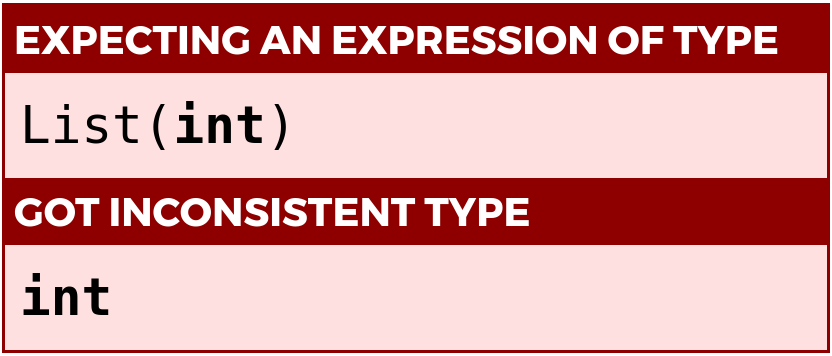
\includegraphics[width=0.28\textwidth,interpolate=false,valign=t]{images/type-inconsistency.png}
\vspace{2px}
\caption{Example 3: Ill-Typed Quicksort}
\label{fig:qsort-type-error}
\vspace{-3px}
\end{figure}
% \end{subfigure}


The previous examples were incomplete 
because of \emph{missing} expressions.
%
Now, we discuss programs that are incomplete, 
and therefore conventionally meaningless, because of
\emph{type inconsistencies}. 
%
Let us return to the quicksort example just described, 
but assume that the programmer has filled in the previous hole
as shown in Fig.~\ref{fig:qsort-type-error}. In Sec.~\ref{sec:resumption}, we discuss
how the programming environment could avoid restarting evaluation after such edits by using the values stored in the hole closures.

The programmer appears to be on the right track conceptually
in recognizing that the pivot needs to appear between the 
smaller and bigger elements. 
However, the types do not quite work out: the \li{@} operator here
performs list concatenation, but the pivot is an integer. 
Most compilers and editors will report a static error message
to the programmer in this case, and \Hazel 
follows suit in the type inspector (shown inset in Fig.~\ref{fig:qsort-type-error}). 
However, our argument is that the presence of a static type error should not cause all feedback about 
the dynamic behavior of the program to ``flicker out'' or ``go stale'' --
after all, there are perfectly meaningful parts of the program (both nearby
and far away from the error) 
whose dynamic behavior may be of interest. Concrete results can also help the programmer understand the implications of the type error \cite{Seidel2016}.
% After all,
% the error is localized and there is perfectly good code elsewhere 
% in the program (if not nearby, then perhaps far away).

Our approach, following the prior work of \citet{popl-paper}, 
is to semantically internalize the ``red outline'' around
a type-inconsistent expression as a \emph{non-empty hole} around that expression.
Evaluation safely proceeds past a non-empty hole just as if it were an empty hole.
The semantics also associates an environment with each instance of a non-empty hole,
so we can use the live context inspector essentially as in Fig.~\ref{fig:qsort-sidebars} (not shown). 
Evaluation proceeds inside the hole, so that 
feedback about the type-inconsistent expression, which might ``almost'' be correct, is available. 
In this case, the result at the bottom of Fig.~\ref{fig:qsort-type-error}
reveals that the programmer is on the right track: the list elements 
appear in the correct order.
They simply have not been combined correctly.

We are treating \li{@} as a primitive operator in this example. If it were defined as a function, then
it would be possible to further reduce the example by proceeding into the function body. This is likely unhelpful for
functions other than those that programmer is actively working on. Our semantics \emph{allows} beta reduction when the argument is a hole, but it does not \emph{require} it.

Although \Hazel inserts non-empty holes automatically, the earlier work on \Hazelnut allowed the programmer to explicitly insert non-empty holes. It may be that these are useful even when there is not a type inconsistency because the non-empty hole defers elimination of the enclosed expression and causes hole closure information to be tracked. For example, if we repaired the program in Fig.~\ref{fig:qsort-type-error} by replacing the erroneous variable \li{pivot} with \li{[pivot]} and then inserted a non-empty hole around this expression, the result would show all of the list concatenation operations that would be performed without actually performing them, producing a result much like that in Fig.~\ref{fig:qsort-type-error}. This provides another way to explore the recursive structure of the \li{qsort} function.

% For example, consider the following two definitions.

% \begin{lstlisting}
% let bad_bool : bool = ?? 0 ??_bad_bool;

% let bad_int : int = 1 + ?? true ??_bad_int_second_argument;
% \end{lstlisting}

% \noindent
% %
% These two definitions are ill-typed under standard typing disciplines.
% %
% In contrast, \citet{popl-paper} present a bidirectional type system that assigns
% types to both, by wrapping type-inconsistent expressions (\li{0} on line
% \rkc{XXX} and \li{true} on line \rkc{XXX} above) in \emph{non-empty} holes.
% %
% Non-empty holes prevent local type inconsistencies from polluting the rest of
% the program surrounding it, which may or may not itself contain additional
% inconsistencies.

\begin{comment}
\overviewExample{2}{Sum List}
%
Consider the following buggy program (observed during an undergraduate
functional programming course~\cite{Seidel2016}) that attempts to sum a list
integers.
%
The error is that the base case produces a list rather than an integer.

\begin{lstlisting}
sum_list : list(int) -> int
sum_list [] = ?[]?
sum_list (n:ns) = n + sum_list ns
\end{lstlisting}

\noindent
%
Because the list expression on line 2 does not have type \li{int} as required,
it is wrapped in a (non-empty) hole by the bidirectional type
checker~\cite{popl-paper}.
%
Rather than trying to debug the error based on the static error, the programmer
may wish to trying running the function anyway by calling, say, \li{sum_list(2)}.
%
\HazelnutLive{} runs and produces the indeterminate expression \li{3 + ?[]?}.
%
By observing that the hole expression is being added to the integer \li{3}, he
realizes that it needs to be an integer, specifically, \li{0}.
%
Compared to the trace displayed by \citet{Seidel2016}, the indeterminate result
produced by \HazelnutLive{} is ``flattened'' because the expression \li{1 + 2}
successfully proceeded to evaluate despite the error elsewhere.
\end{comment}

%% TODO fold error from Erwig paper.
%% %
%% see that final call on stack does have the right answer, but
%% it's wrapped in a singleton list when the expected type is not
%% a list.
%% %
%% fix is to remove the list, the rest of the computation remains
%% the same, but b/c they were all wrapped in holes, need to re-run.
%% %
%% (add some mechanism for type-consistent non-empty-holes...)

\begin{comment}

\overviewExample{4}{Stutter}
%
Consider the following function which attempts to produce a
list where every element is repeated twice (borrowed from \citet{Osera2015}).
%
The combiner function to \li{List.foldr} needs to produce a \li{list(int)}, but
it produces a \li{list(list(int)} instead.

\begin{lstlisting}
stutter : list(int) -> list(int)
stutter xs = List.foldr (\x acc -> ?[x,x]? : acc) [] xs
\end{lstlisting}

\noindent
%
The bidirectional type checker of \citet{popl-paper} wraps the expression
\li{[x,x]} inside a non-empty hole.
%
%% The editor has a choice about which expression to ``blame'' for the error; the
%% entire application that forms the body of the lambda is analyzed against the
%% return type \li{list(int)}, so that is a reasonable choice for the editor to
%% make; another would be to assume that the arguments \li{[x,x]} and \li{acc} are
%% both as intended and that only the function \li{(:)} is type-consistent.
%% %
%% Although one could imagine a setting in which a user would perform this
%% reasoning, let's assume the simplest approach for marking consistencies that
%% wraps the entire application.
%
Running this on \li{stutter [1,2,3]} produces the indeterminate result

\begin{lstlisting}
?  [1,1] : (? [2,2] : (? [[3:3]] ?) ?) ?,
\end{lstlisting}

\noindent
%
which shows the unfolding of \li{List.foldr}.
%
We refer to nested indeterminate computations like this as \rkc{\emph{hole
environment traces} or \emph{hole environment trees}}.
%
The result of the innermost indeterminate expression is \li{[[3,3]]}.
%
The user realizes that there are too many levels of nesting, so
he replaces the \li{(:)} with \li{(@)}, which addresses the type inconsistency
and, when reevaluated, produces the desired result.

\end{comment}

% !TEX root = hazelnut-dynamics.tex

\subsection{Example 4: Type Holes and Dynamic Type Errors}
\label{sec:dynamic-type-errors}

% \begin{subfigure}[t]{\textwidth}
\begin{figure}
\centering
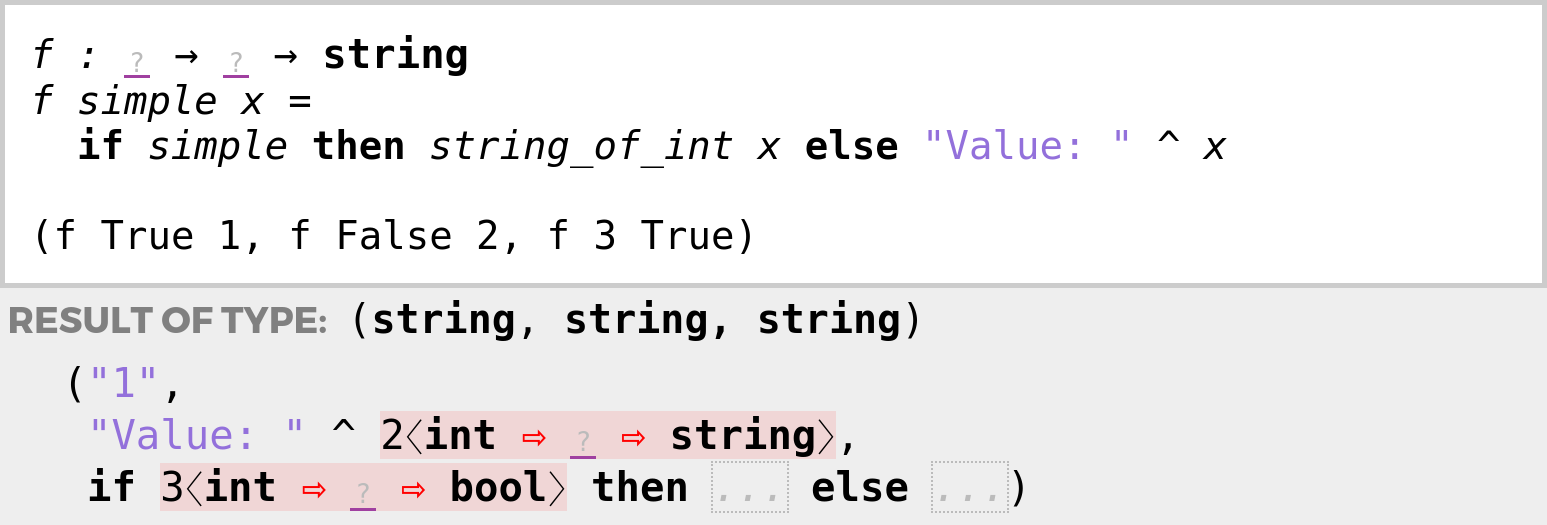
\includegraphics[width=0.73\textwidth,interpolate=false,valign=t]{images/cast-errors.png}
% 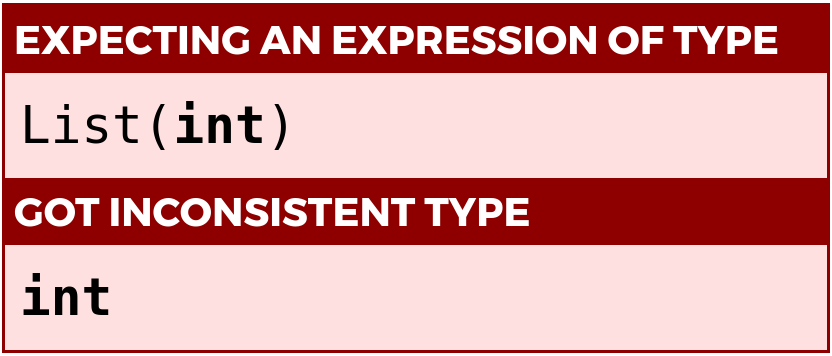
\includegraphics[width=0.28\textwidth,interpolate=false,valign=t]{images/type-inconsistency.png}
\caption{Example 4: Type Holes and Dynamic Type Errors}
\label{fig:cast-errors}
\vspace{-6px}
\end{figure}
% \end{subfigure}


% So far, we have only discussed incomplete programs where a hole appears within an expression.
In \Hazel, the program can also be incomplete because holes appear in types. 
\citet{popl-paper} confirmed that the literature on \emph{gradual type systems} \cite{Siek06a,DBLP:conf/snapl/SiekVCB15} is directly relevant to the problem of reasoning statically with type holes, by identifying the type hole with the unknown type. 
Unsurprisingly, then, it is also relevant to the problem of running 
programs with type holes. Indeed, that is the purpose of gradual typing: to be able to run programs that are not yet sufficiently annotated with types by inserting \emph{casts} only where necessary. As such, let us consider only a small synthetic example to demonstrate what is unique to our approach.

Fig.~\ref{fig:cast-errors} defines a simple function, \li{f}, of two arguments. 
The type annotation on the first line leaves the type of those arguments unknown. 
As such, the \Hazel type system, following the gradual typing approach,
allows the body of the function to use those two
arguments at any type at all (that is, the hole type is universally consistent). 
In this case, the first argument, \li{simple}, is used at one type, \li{bool}, 
and the second argument, \li{x}, is used at two different types in the two branches (perhaps because the programmer made a mistake), 
first as an \li{int} and second as a \li{string}  (we use \li{^} for string concatenation).
Although \Hazel supports only local type inference as of this writing, 
a system that uses ML-style type reconstruction to fill type holes statically, like GHC Haskell, would only be able to fill the first hole. Leaving the second hole unfilled is 
a parsimonious alternative to arbitrarily or heuristically\todo{cite error localization papers?}{} choosing one of the possibilities and marking the
other uses of \li{x} as ill-typed.

At the bottom of the cell in Fig.~\ref{fig:cast-errors}, we have three 
example applications of \li{f}. In this case, we simply tuple the results, but we could also
have made them into tests or put them into separate cells. All three are statically
well-typed, again because the hole type is universally consistent.
The result at the bottom of Fig.~\ref{fig:cast-errors} demonstrates that the first application
of \li{f} is dynamically unproblematic. This might help the programmer confirm that at least
the first branch of the function body has been implemented as intended without the need to comprehensively
address all of the problems in the program. This flexibility is a common motivation for dynamic languages in programming folklore.

The second application of \li{f}, in contrast, causes a dynamic type error because the second argument, \li{2}, is an \li{int} but evaluation takes the branch where \li{x} is used as a \li{string}. 
Rather than aborting evaluation immediately when this occurs, as in existing gradual type systems, the problematic sub-term becomes a \emph{failed cast} term, shown shaded in red, which can be read ``\li{2} is an \li{int} that was used through a variable of hole type (\li{?}) as a \li{string}''. 
A failed cast behaves much like a non-empty hole in that it simply becomes an opaque value of the target type, \li{string}, that causes the surrounding concatenation operation to become indeterminate. 
Evaluation can continue on to the third application of \li{f}, which again is problematic, this time because the first argument is not a \li{bool} (perhaps because the programmer had an incorrect understanding of the argument order). 
Again, this causes a failed cast to appear, this time in guard position. Like a hole in guard position, evaluation cannot determine which branch to take so the whole guard expression becomes indeterminate. 
The pretty printer
hides the two branches behind ellipses.

In this synthetic example, it might have only been a small burden for the programmer to provide the intended types in the signature of \li{f}, but there are situations (e.g. during rapid prototyping or a live performance) where the programmer may consider the burden more substantial. This approach ensures that dynamic feedback does not have gaps even when there is a dynamic type error.

\subsection{Design Variations}


\begin{comment}
\emph{Gradual type systems}~(\eg{}~\cite{XXX,XXX,XXX}) can statically accept
programs that would otherwise be rejected by static type systems---either
because type inference cannot reconstruct a valid type assignment, or because
there may not be a unique valid type assignment at all.
%
In either case, gradual type systems allow types to contain \emph{unknown
types}, and partially unknown types can be used in contexts that require
different types, so long as they are \emph{consistent} (intuitively, equal
modulo the unknown parts).
%
Dynamic casts are then inserted to ensure that these remaining static
discrepancies are not violated at run-time.

\HazelnutLive{} inherits the notion of \emph{type holes} from
\citet{popl-paper}, which serves a similar static purpose as the unknown type in
gradual type systems.
%
In contrast to prior gradually typed languages, however, \HazelnutLive{} can
evaluate ``around'' cast errors in the same way as it does for expression holes.

\overviewExample{3}{Dynamically Typed Negation}

Consider the \li{negate} function (adapted from \cite{ChughPOPL2012}), which
cannot be assigned a static type in a conventional type system---either a
bidirectional one, like in \HazelnutLive{}, or one with ML-style,
unification-based inference---because the argument \li{x} is used at type
\li{int} on line \rkc{XXX} and \li{bool} on line \rkc{XXX}.
%
Therefore, the declared type of \li{x} is the hole type \li{??}, which allows
\li{x} to be used at the conflicting types, with each use expanded into an
expression wrapped in a \emph{cast} that will dynamically check for safety.
%
The return type also uses the hole type \li{??}, leading to additional casts in
the expansion.

\begin{lstlisting}
negate : bool -> ?? -> ??
negate b x =
  if b
    then 0 - x     // expanded to: (0 - (x<?? => int>))<int => ??>
    else not x     // expanded to: (not (x<?? => bool>))<bool => ??>

(negate false 1) + 2 + 3 + (negate true 4)
\end{lstlisting}

\noindent
%
As in prior gradually typed languages~\cite{XXX},
evaluating the expression \li{negate false 1} on line \rkc{XXX} leads to
\li{(not (1<int => ??><?? => bool>))<bool => ??>}, where the inner casts
lead to the \emph{cast error} \li{1<?? =/=> bool>} because \li{1} cannot be
safely treated as having type \li{bool}.
%
Unlike in prior gradually typed languages, however, \HazelnutLive{} evaluates
around the cast error, making progress on the \li{2 + 3 + negate false 4}
expression that surrounds the error; the final indeterminate result is
\li{(not (1<?? =/=> bool>))<bool => ??> + 1}.
%
Just like it is useful for static type checkers to report multiple errors, our
approach allows us to report multiple dynamic cast errors, and otherwise make
progress on expressions that do not depend on failed casts.
%
This approach can be incorporated into existing gradually typed languages.
\end{comment}
\begin{comment}
\subsection{Live Programming for Debugging}

Previous examples highlighted how running different kinds of incomplete
programs---ones with missing expressions, type-inconsistent expressions, or
missing types---can be useful.
%
Our final example demonstrates how expression holes may be useful even for
complete programs, in order to facilitate debugging and program understanding.

%% \overviewExample{6}{\rkc{...}}
%%
%% \rkc{breakpoints, understanding input/output behavior}

\overviewExample{4}{Quicksort}

Consider the following buggy implementation of quicksort, which contains several
errors.
%
The student wants to debug the implementation and so inserts an expression
around the return expression on line \rkc{XXX}, and runs
\li{quicksort [X,X,X,X,X,X]}.

\begin{lstlisting}
quicksort : list('a) -> list('a)
quicksort [] = []
quicksort (x:xs) =
  let (left, right) = span ((>) x) xs in
  let (left', right') = (quicksort left, quicksort right) in
  ? (left' @ [x] @ right) ?
\end{lstlisting}

\noindent
%
Based on the live environment for the initial call, the student notices that the
values in \li{left} are larger than the pivot \li{x}, but \li{left} was intended
to bind smaller values.
%
This suggests that the student got the filtering predicate backwards, so he
replaces it with \li{(<)} on line \rkc{XXX}.
%
After re-running the program and viewing the live output again, \li{left} now
contains smaller values than \li{x}, but not all of them; \li{right} has some
values that are larger and some that are smaller.
%
The student uses type-based search to find other functions, besides \li{span},
of type \li{('a -> bool) -> 'a list -> ('a list, 'a list)} and finds
\li{partition}.
%
It may be easier for the student to simply try the function rather than studying
the documentation, so he edits line \rkc{XXX} to call \li{partition} instead,
re-runs, and observes that both \li{left} and \li{right} now seem to achieve the
intended partitioning.

Despite these two fixes, the result expression is not yet sorted.
%
In particular, the values greater than the pivot \li{x} are not completely
sorted.
%
Viewing the values of bindings of \li{left'} and \li{right'}, the student sees
that both seem to have correct prefixes of sorted lists, but that they are
incorrect after the pivots.
%
This suggests that something may be wrong with the handling of \li{right'}.
%
Indeed, the student takes a look for uses of \li{right'} and sees that line
\rkc{XXX} mistakenly uses \li{right} instead.
%
Making this change and re-running now produces the desired result, built up as a
hole environment tree that shows how all of the recursive results will be
combined by a series of nested appends.
%
Happy with the results of the program, the student removes the hole around the
expression on line \rkc{XXX}, and evaluation can proceed to perform the nested
appends, producing the final sorted result.
%
\autoref{sec:discussion} discusses how debugging tools may be designed to
systematically insert hole expressions in particular places to achieve certain
debugging and program understanding strategies.
%
%% When run on a larger input, this projection of the full evaluation trace shows a
%% nesting structure---which could be rendered as visualization to help
%% understanding, as described in \autoref{sec:discussion}---whose depth is clearly
%% much smaller than the length of the input list; this suggests that the
%% algorithm, indeed, achieves some sort of sublinear complexity, as intended.
%

\begin{lstlisting}
quicksort : list('a) -> list('a)
quicksort [] = []
quicksort (x:xs) =
  let (left, right) = partition ((<) x) xs in
  let (left', right') = (quicksort left, quicksort right) in
  ? (left' @ [x] @ right') ?
\end{lstlisting}
\end{comment}



% \paragraph{Recap}
% %
% In the above four subsections, respectively, we considered programs with:
% %
% (1) empty expression holes,
% %
% (2) non-empty expression holes for ill-typed expressions,
% %
% (3) type holes, and
% %
% (4) non-empty expression holes for well-typed expressions.
% %
% Next, we will formally describe the novel dynamic semantics of \HazelnutLive{}
% that allows programs with combinations of these kinds of incompleteness to be
% evaluated.
